% Options for packages loaded elsewhere
\PassOptionsToPackage{unicode}{hyperref}
\PassOptionsToPackage{hyphens}{url}
\PassOptionsToPackage{dvipsnames,svgnames,x11names}{xcolor}
%
\documentclass[
  letterpaper,
  DIV=11,
  numbers=noendperiod]{scrartcl}

\usepackage{amsmath,amssymb}
\usepackage{iftex}
\ifPDFTeX
  \usepackage[T1]{fontenc}
  \usepackage[utf8]{inputenc}
  \usepackage{textcomp} % provide euro and other symbols
\else % if luatex or xetex
  \usepackage{unicode-math}
  \defaultfontfeatures{Scale=MatchLowercase}
  \defaultfontfeatures[\rmfamily]{Ligatures=TeX,Scale=1}
\fi
\usepackage{lmodern}
\ifPDFTeX\else  
    % xetex/luatex font selection
\fi
% Use upquote if available, for straight quotes in verbatim environments
\IfFileExists{upquote.sty}{\usepackage{upquote}}{}
\IfFileExists{microtype.sty}{% use microtype if available
  \usepackage[]{microtype}
  \UseMicrotypeSet[protrusion]{basicmath} % disable protrusion for tt fonts
}{}
\makeatletter
\@ifundefined{KOMAClassName}{% if non-KOMA class
  \IfFileExists{parskip.sty}{%
    \usepackage{parskip}
  }{% else
    \setlength{\parindent}{0pt}
    \setlength{\parskip}{6pt plus 2pt minus 1pt}}
}{% if KOMA class
  \KOMAoptions{parskip=half}}
\makeatother
\usepackage{xcolor}
\setlength{\emergencystretch}{3em} % prevent overfull lines
\setcounter{secnumdepth}{-\maxdimen} % remove section numbering
% Make \paragraph and \subparagraph free-standing
\ifx\paragraph\undefined\else
  \let\oldparagraph\paragraph
  \renewcommand{\paragraph}[1]{\oldparagraph{#1}\mbox{}}
\fi
\ifx\subparagraph\undefined\else
  \let\oldsubparagraph\subparagraph
  \renewcommand{\subparagraph}[1]{\oldsubparagraph{#1}\mbox{}}
\fi


\providecommand{\tightlist}{%
  \setlength{\itemsep}{0pt}\setlength{\parskip}{0pt}}\usepackage{longtable,booktabs,array}
\usepackage{calc} % for calculating minipage widths
% Correct order of tables after \paragraph or \subparagraph
\usepackage{etoolbox}
\makeatletter
\patchcmd\longtable{\par}{\if@noskipsec\mbox{}\fi\par}{}{}
\makeatother
% Allow footnotes in longtable head/foot
\IfFileExists{footnotehyper.sty}{\usepackage{footnotehyper}}{\usepackage{footnote}}
\makesavenoteenv{longtable}
\usepackage{graphicx}
\makeatletter
\def\maxwidth{\ifdim\Gin@nat@width>\linewidth\linewidth\else\Gin@nat@width\fi}
\def\maxheight{\ifdim\Gin@nat@height>\textheight\textheight\else\Gin@nat@height\fi}
\makeatother
% Scale images if necessary, so that they will not overflow the page
% margins by default, and it is still possible to overwrite the defaults
% using explicit options in \includegraphics[width, height, ...]{}
\setkeys{Gin}{width=\maxwidth,height=\maxheight,keepaspectratio}
% Set default figure placement to htbp
\makeatletter
\def\fps@figure{htbp}
\makeatother

\KOMAoption{captions}{tableheading}
\makeatletter
\makeatother
\makeatletter
\makeatother
\makeatletter
\@ifpackageloaded{caption}{}{\usepackage{caption}}
\AtBeginDocument{%
\ifdefined\contentsname
  \renewcommand*\contentsname{Table of contents}
\else
  \newcommand\contentsname{Table of contents}
\fi
\ifdefined\listfigurename
  \renewcommand*\listfigurename{List of Figures}
\else
  \newcommand\listfigurename{List of Figures}
\fi
\ifdefined\listtablename
  \renewcommand*\listtablename{List of Tables}
\else
  \newcommand\listtablename{List of Tables}
\fi
\ifdefined\figurename
  \renewcommand*\figurename{Figure}
\else
  \newcommand\figurename{Figure}
\fi
\ifdefined\tablename
  \renewcommand*\tablename{Table}
\else
  \newcommand\tablename{Table}
\fi
}
\@ifpackageloaded{float}{}{\usepackage{float}}
\floatstyle{ruled}
\@ifundefined{c@chapter}{\newfloat{codelisting}{h}{lop}}{\newfloat{codelisting}{h}{lop}[chapter]}
\floatname{codelisting}{Listing}
\newcommand*\listoflistings{\listof{codelisting}{List of Listings}}
\makeatother
\makeatletter
\@ifpackageloaded{caption}{}{\usepackage{caption}}
\@ifpackageloaded{subcaption}{}{\usepackage{subcaption}}
\makeatother
\makeatletter
\@ifpackageloaded{tcolorbox}{}{\usepackage[skins,breakable]{tcolorbox}}
\makeatother
\makeatletter
\@ifundefined{shadecolor}{\definecolor{shadecolor}{rgb}{.97, .97, .97}}
\makeatother
\makeatletter
\makeatother
\makeatletter
\makeatother
\ifLuaTeX
  \usepackage{selnolig}  % disable illegal ligatures
\fi
\IfFileExists{bookmark.sty}{\usepackage{bookmark}}{\usepackage{hyperref}}
\IfFileExists{xurl.sty}{\usepackage{xurl}}{} % add URL line breaks if available
\urlstyle{same} % disable monospaced font for URLs
\hypersetup{
  pdftitle={Activity: Paintings catalogue in Jupyter Notebook},
  colorlinks=true,
  linkcolor={blue},
  filecolor={Maroon},
  citecolor={Blue},
  urlcolor={Blue},
  pdfcreator={LaTeX via pandoc}}

\title{Activity: Paintings catalogue in Jupyter Notebook}
\author{}
\date{}

\begin{document}
\maketitle
\ifdefined\Shaded\renewenvironment{Shaded}{\begin{tcolorbox}[enhanced, interior hidden, sharp corners, frame hidden, boxrule=0pt, breakable, borderline west={3pt}{0pt}{shadecolor}]}{\end{tcolorbox}}\fi

Objective: Make a selection of nine paintings for the exhibition
catalogue to be selected from Wikidata and rendered multi-format in
Quarto.

The below Python code uses SPARQLWrapper to retrieve data from Wikidata
based on a SPARQL query.

Requirement already satisfied: SPARQLWrapper in
c:\users\lisas\appdata\local\programs\python\python311\lib\site-packages
(2.0.0) Requirement already satisfied: rdflib\textgreater=6.1.1 in
c:\users\lisas\appdata\local\programs\python\python311\lib\site-packages
(from SPARQLWrapper) (6.3.2) Requirement already satisfied:
isodate\textless0.7.0,\textgreater=0.6.0 in
c:\users\lisas\appdata\local\programs\python\python311\lib\site-packages
(from rdflib\textgreater=6.1.1-\textgreater SPARQLWrapper) (0.6.1)
Requirement already satisfied: pyparsing\textless4,\textgreater=2.1.0 in
c:\users\lisas\appdata\local\programs\python\python311\lib\site-packages
(from rdflib\textgreater=6.1.1-\textgreater SPARQLWrapper) (3.0.9)
Requirement already satisfied: six in
c:\users\lisas\appdata\local\programs\python\python311\lib\site-packages
(from
isodate\textless0.7.0,\textgreater=0.6.0-\textgreater rdflib\textgreater=6.1.1-\textgreater SPARQLWrapper)
(1.16.0)

Wikidata link: \url{http://www.wikidata.org/entity/Q18683025}

Title: Ballsouper

Creator: Adolph von Menzel

Year: 1878-01-01T00:00:00Z

Inventory number: A I 902

Copyright: Gemeinfreiheit

Material: Leinwand

Wikidata link: \url{http://www.wikidata.org/entity/Q18683025}

Title: Das Ballsouper

Creator: Adolph von Menzel

Year: 1878-01-01T00:00:00Z

Inventory number: A I 902

Copyright: Gemeinfreiheit

Material: Ölfarbe

Wikidata link: \url{http://www.wikidata.org/entity/Q18683025}

Title: Das Ballsouper

Creator: Adolph von Menzel

Year: 1878-01-01T00:00:00Z

Inventory number: A I 902

Copyright: Gemeinfreiheit

Material: Leinwand

Wikidata link: \url{http://www.wikidata.org/entity/Q18683026}

Title: Eisenwalzwerk

Creator: Adolph von Menzel

Year: 1875-01-01T00:00:00Z

Inventory number: A I 201

Copyright: Gemeinfreiheit

Material: Ölfarbe

Wikidata link: \url{http://www.wikidata.org/entity/Q18683026}

Title: Eisenwalzwerk

Creator: Adolph von Menzel

Year: 1875-01-01T00:00:00Z

Inventory number: A I 201

Copyright: Gemeinfreiheit

Material: Leinwand

Wikidata link: \url{http://www.wikidata.org/entity/Q18683026}

Title: Eisenwalzwerk (Moderne Cyklopen)

Creator: Adolph von Menzel

Year: 1875-01-01T00:00:00Z

Inventory number: A I 201

Copyright: Gemeinfreiheit

Material: Ölfarbe

Wikidata link: \url{http://www.wikidata.org/entity/Q18683026}

Title: Eisenwalzwerk (Moderne Cyklopen)

Creator: Adolph von Menzel

Year: 1875-01-01T00:00:00Z

Inventory number: A I 201

Copyright: Gemeinfreiheit

Material: Leinwand

Wikidata link: \url{http://www.wikidata.org/entity/Q18683032}

Title: Waldbrunnen bei Ariccia

Creator: Ludwig Richter

Year: 1831-01-01T00:00:00Z

Inventory number: A III 781

Copyright: Gemeinfreiheit

Material: Ölfarbe

Wikidata link: \url{http://www.wikidata.org/entity/Q232084}

Title: Zwei Männer am Meer

Creator: Caspar David Friedrich

Year: 1817-01-01T00:00:00Z

Inventory number: A II 884

Copyright: Gemeinfreiheit

Material: Ölfarbe

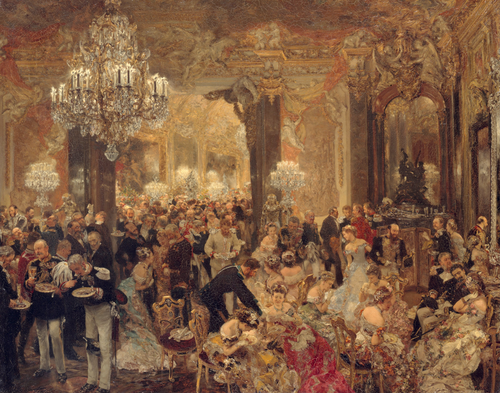
\includegraphics{paintingsSommer_files/figure-pdf/cell-5-output-2.png}\hspace{-26pt}
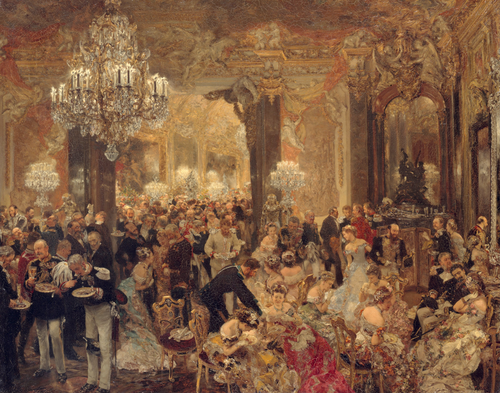
\includegraphics{paintingsSommer_files/figure-pdf/cell-5-output-3.png}
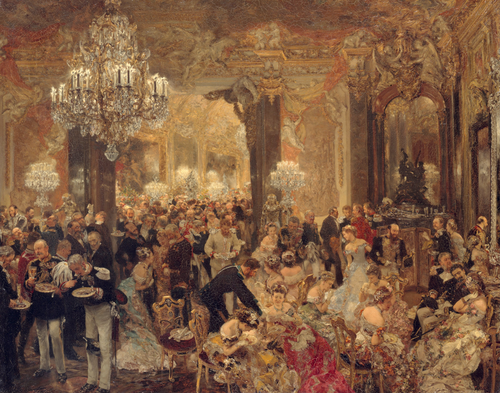
\includegraphics{paintingsSommer_files/figure-pdf/cell-5-output-4.png}
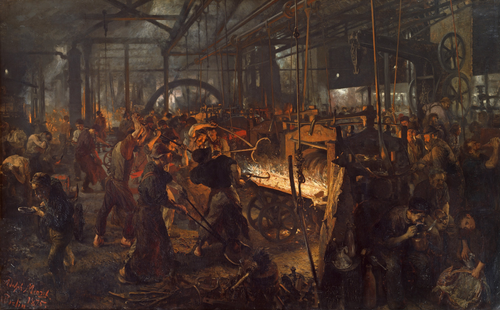
\includegraphics{paintingsSommer_files/figure-pdf/cell-5-output-5.png}
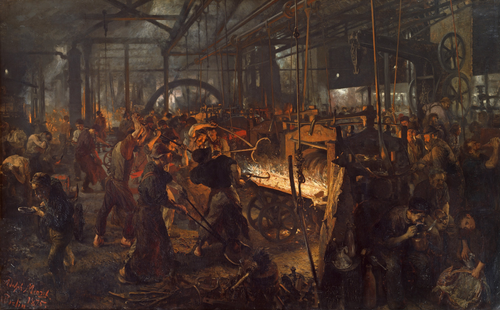
\includegraphics{paintingsSommer_files/figure-pdf/cell-5-output-6.png}
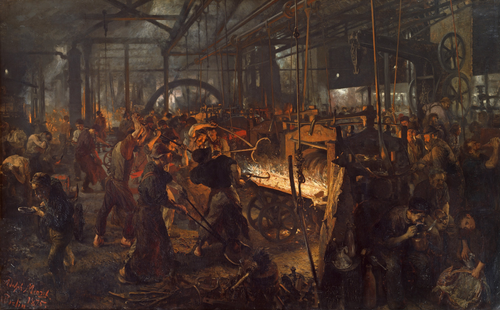
\includegraphics{paintingsSommer_files/figure-pdf/cell-5-output-7.png}
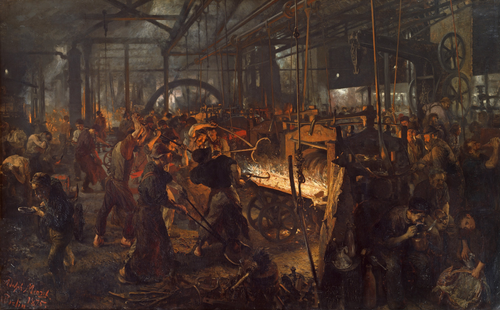
\includegraphics{paintingsSommer_files/figure-pdf/cell-5-output-8.png}
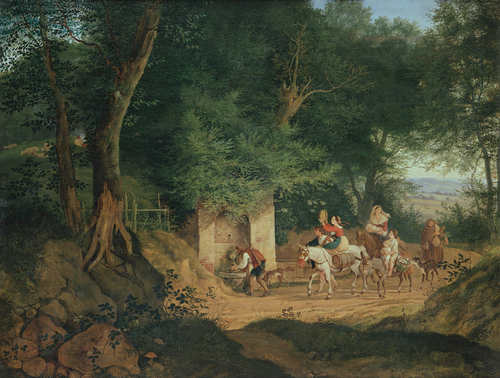
\includegraphics{paintingsSommer_files/figure-pdf/cell-5-output-9.png}
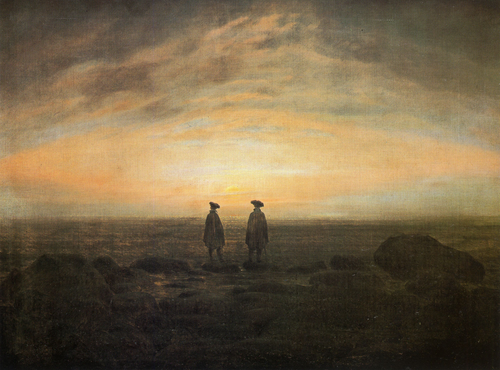
\includegraphics{paintingsSommer_files/figure-pdf/cell-5-output-10.png}



\end{document}
